
\label{sec:systemArchitecture}

	
 

\subsection{Klassendiagramm}

\begin{figure}[!h]
	 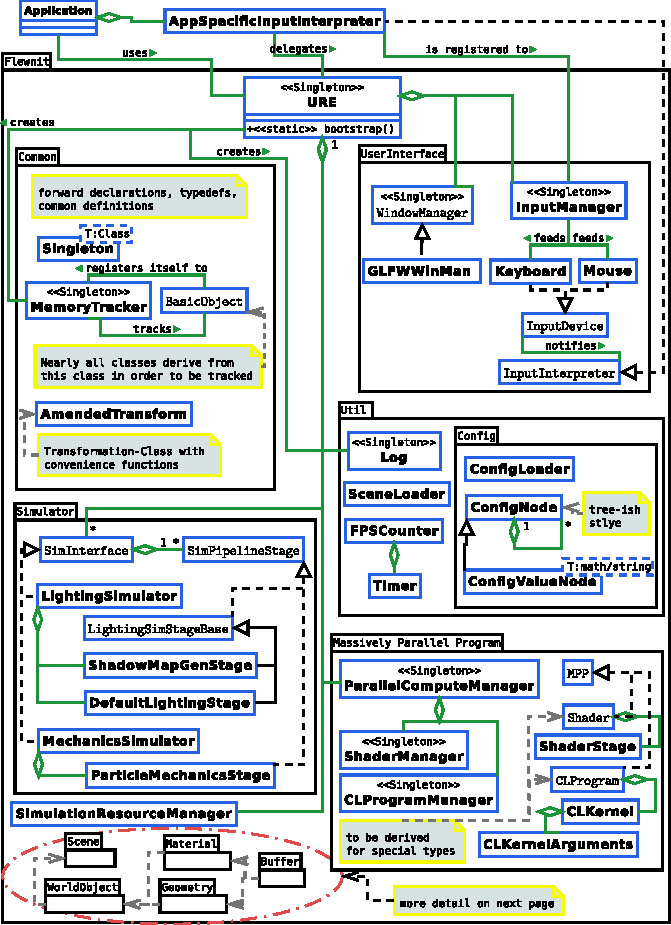
\includegraphics[width=\textwidth]{Overview_Flewnit_Architecture_After_Implementation1.pdf}
	\caption{Klassendiagramm des Gesamtsystems, Teil 1}
	\label{fig:ClassDiagOverview1}
\end{figure}



\subsection{Dependencies}
	\label{sec:dependencies}

		
	\subsubsection{OpenGL3/4}
	
	- verwendung von mindestens OpenGL 3/3 core context, um legacy code schon zur compilezeit auszuschließen
	
	
    \subsubsection{OpenCL 1.0}
    	noch keine offenen openCL 1.1 treiber, außerdem keine features davon benötigt;
    	c++-wrapper genutzt, auch von khronos-seiten beziehbar;
    	Gegenüberstellung zu CUDA, vor- und nachteile auflisten, insbesondere das problem ,dass esk ein 1D-texturen in OpenCL gibt, und man sich entscheiden muss zwischen generischem buffer und Textur, man also nicht hin und her-interpretieren kann wie in CUDA;
    
    
    \subsubsection{GLFW}
    	Fenstermanager + input
    	explizite GL3 core profile creation, einfaches fullscreen, multisampling, keine mainloop, explizites input pulling, 
    	mouse grab, alles viel besser als GLUT :)
    \subsubsection{Grantlee}
       die string template engine die CL und GL code erzeugt
    \subsubsection{assimp}
    \subsubsection{ogl math}
    	leichte, aber doch recht maechtige mathe-bibliothek
    \subsubsection{TinyXML}
    - möglichst hohe Konfiguriertbarkeit ohne ständigen recompile: parsing von XML config file
    	
 
\subsection{BasicObject und Memory Tracking}
	 für vielseitig, flexible anwendung zur Laufzeit sollten keine 	Speicher-Lecks auftreten damit Funktionalität 
	 kontrolliert heruntergefahren und neu initialisiert werden kann; 
	 	- memory tracking, (erklären, warum nicht tracking mit Valgrind)
 
    	
\subsection{Die \emph{Unified Rendering Engine}}
URE blubb

\subsection{Die Simulator-Klassen}


\subsection{Die SimulationPipelineStages}
	shdow map gen, direct lighting, rendering features particlemechanics stage;
	in planung: deferred rendering G-Bufferfill, deferred rendering shade, div. post processing stages


\subsection{Die Manager-Klassen}
Für gemeinsamen zugriff sollten viele Daten für andere Klassen verfügbar sein (Buffer, Rendering Results...); 	
Realisierung über Manager-Singleton-Klassen und Zugriff über Map-Container;
\todo[color=green]{evtl. andere reihenfolge}

\subsection{Die Template-Engine}
	\label{sec:architecture:templateEngine}
	exemplarischer code schnipsel, refernz su shadermanager und CLProgramManager, erklärung wie man templat contex setzt, 	
	vererbung etc;
    	
\subsection{Die Buffer-Abstraktion}  
	\label{sec:architecture:BufferAbstraction} 	
 	die bombe, die cpu, ogl und ocl vereint, inclusive ping ponging etc.. 
 	fundamentale Klassensammlung fuer den Unified-Aspekt
 	
 	\begin{figure}[!h]
  		\begin{tabular}
  		{
  		 l  l | c | c | c |
  		}
																	\cline{3-5}
  									&								&	\multicolumn{3}{ c | }{Context} \\ 
  																	\cline{3-5}
									&								& 	Host 	& 	OpenGL 	& 	OpenCL	\\
    	\noalign{\hrule}								
    	\multicolumn{1}{|c|}{
    		generic Buffer
    	}							& 								
    		&	{\color{green}\checkmark} 	&	{\color{red}x}		& 	{\color{green}\checkmark}	\\ 
    	
    	\noalign{\hrule}								
    	\multicolumn{1}{|c|}{
    		\multirow{4}{*}{OpenGL Buffers}
    	}							& Vertex Attribute Buffer		
    		&	{\color{orange}o} 	&	{\color{green}\checkmark}		& 	{\color{orange}o}	\\  
    								\cline{3-5}
    	\multicolumn{1}{|c|}{}		& Vertex Index Buffer			
    		&	{\color{orange}o} 	&	{\color{green}\checkmark}		& 	{\color{orange}o}	\\  
    								\cline{3-5}
    	\multicolumn{1}{|c|}{}		& Uniform Buffer
    		&	{\color{orange}o} 	&	{\color{green}\checkmark}		& 	{\color{orange}o}	\\ 
    								\cline{3-5} 
    	\multicolumn{1}{|c|}{}		& Render Buffer					
    		&	{\color{red}x} 	&	{\color{green}\checkmark}		& 	{\color{green}\checkmark}	\\ 
    
   		\noalign{\hrule}								
   		\multicolumn{1}{|c|}{
    		\multirow{4}{*}{Textures} 
   		}							& 1D Texture					
   			&	{\color{orange}o} 	&	{\color{green}\checkmark}		& 	{\color{red}x}	\\ 
    								\cline{3-5}
		\multicolumn{1}{|c|}{}		& 2D Texture				
			&	{\color{orange}o} 	&	{\color{green}\checkmark}		& 	{\color{green}\checkmark}	\\ 
									\cline{3-5}
		\multicolumn{1}{|c|}{}		& 3D Texture		
			&	{\color{orange}o} 	&	{\color{green}\checkmark}		& 	{\color{green}\checkmark}	\\ 
									\cline{3-5}
		\multicolumn{1}{|c|}{}		& Special Texture				
			&	{\color{orange}?} 	&	{\color{green}\checkmark}		& 	{\color{orange}?}	\\ 


    	\noalign{\hrule}
     
     	
  		\end{tabular}	
  	
  		\caption{		
  			Verschiedene Buffertypen und ihre Verfügbarkeit in verschiedenen Kontexten \\	
  			Legende: \\
			{\color{green}\checkmark}	$\rightarrow$ nativ unterstützt;
			{\color{orange}o}	$\rightarrow$ kompatibel;
			{\color{red}x}	$\rightarrow$ nicht unterstützt;	\\
			{\color{orange}?}	$\rightarrow$ Unterstützung abhängig von weiteren Parametern;	
		}
	
  	\end{figure}
 
\subsection{Das WorldObject}
	Basis-Klasse fuer alles was unified simuliert wird: pure viuelle objekt, uniform grid, fluid, rigid body etc..
	
	\subsubsection{Das SubObject}
  
 
\subsection{Material}  
	was stellt welches material in welcher Domain dar?
	
\subsection{Geometry}
	Abtract, Buffer based, Vertex based etc.. ein paar konzepte (implementiert/genutzt nur VertexBased)  
	
\subsection{Massively Parallel Program}
	Basisklasse von Shader und OpenCL Program
	\subsubsection{Shader}
		
	\subsubsection{OpenCLProgram}

weitere klassen/konzepte to go...	


\subsection{Status der Implementierung am Ende der BA}
	
	Features auflisten;
	\todo[color=green]{screenshots? oder lieber erst später,zusammen mit detaillierter erläuterung?}

	großteils programmierte, aber ungenutzte/ungetestete features erwähnen (Deferred Rendering, Layered Rendering, 	
	RenderTarget-Klasse, Partikel-Rigid bodies, verschiedene Fluid-Typen); 


	überlegte aber nciht programmierte Konzepte/Algorithmen erwähnen (Triangle-Index-Voxelisierung)
	
	schlimmste schnitzer nennen, wie
		- miese fluid-visualisierung, 
		- unübersichtliche shadertemplates, besser gemacht bei CL-
			Kernel-Templates, 1. weil struktur hier besser "vererbbar", 2. weil mehr erfahrung mit  Template-Engine
	
	  	
  	

\clearpage
